\section{Recursive Least Squares(and Kalman Filter)}
Example 4.4 \; Suppose we have computed the average $\hat{x}_99$ of 99 numbers $b_1,...,b_{99}$. A
new number $b_{100}$ arrives. How can we find the new average $\hat{x}_{100}$ of the 100 b's without
adding the first 99 all over again (plus $b_{100}$)? We want to use only $\hat{x}_99$ and $b_{100}$.

Here is the right combination $\hat{x}_{100}$ of old and new, expressed two ways:
\begin{equation}
New\, average \quad
\hat{x}_{100}=\frac{99}{100}\hat{x}_{99}+\frac{1}{100}b_{100}=\hat{x}_{99}+\frac{1}{100}(b_{100}-\hat{x}_{99})
\end{equation} 
That first term $\frac{99}{100}\hat{x}_{99}$ is $(\frac{99}{100})$ times $(\frac{1}{99})$ times $(b_1+b_2+...+b_{99})$. Canceling 99's, this is $(\frac{1}{100})$ times the sum of 99 b's (without adding them again!). Adding the extra $(\frac{1}{100})$ gives the sum of all b's, divided by 100. This is the correct average.

We prefer the second form of the recursive formula (4.24). The right side is an update
of $\hat{x}_{99}$, by a multiple of the innovation $b_{100}-\hat{x}_{99}$. That innovation tells how much “new information” is in $b_{100}$. When $b_{100}$ equals the old average, the innovation is zero. In that case the updated $\hat{x}_{100}$ is the old $\hat{x}_{99}$, and correction = prediction.

The innovation is multiplied in the update formula (4.24) by $\frac{1}{100}$.This gain factor makes the formula correct. To see the same ideas for Ax = b, start from the least squares solution to an equation $A_{old}x=b_{old}$. New information arrives. There are new measurements $b_{new}$. The combined equation is our Ax = b, to solve by least squares:
\begin{equation}
Combined \,system \quad
\begin{bmatrix}
A_{old} \\ A_{new}
\end{bmatrix}
\begin{bmatrix}
x
\end{bmatrix}
\begin{bmatrix}
b_{old} \\ b_{new}
\end{bmatrix}
lead\,to \quad \hat{x}_{new}.
\end{equation}  
The estimate $\hat{x}_{new}$ comes from this whole system Ax = b. The data in $b_{old}$ still contributes to $\hat{x}_{new}$. But we don't want to do the same calculation twice.

Question 4.1\; Can we update $\hat{x}_{old}$ to $\hat{x}_{new}$, by using only $A_{new}$ and $b_{new}$? Take $C=I$.

Answer\; Since $A^T=\begin{bmatrix} A^T_{old} & A^T_{new}\end{bmatrix}$, we need $A^TA$ in the normal equation:
\begin{equation}
Update\, of\, A^TA \quad
A^TA=A^T_{old}A_{old}+A^T_{new}A_{new}=(known)+(new)
\end{equation}
Then on the right side we need $A^Tb$, also involving old and new:
\begin{equation}
A^Tb=A^T_{old}b_{old}+A^T_{new}b_{new}=A^T_{old}A_{old}\hat{x}_{old}+A^T_{new}b_{new}
\end{equation} 
Substitute $A^TA-A^T_{new}A_{new}$ for $A^T_{old}A_{old}$. Then multiply by $(A^TA)^{-1}$ to find $\hat{x}_{new}$:
\begin{equation*}
\hat{x}_{new}=(A^TA)^{-1}((A^TA-A^T_{new}A_{new})\hat{x}_{old}+A^T_{new}b_{new})
\end{equation*}
This update formula simplifies to produce the new $\hat{x}$ from the old:
\begin{equation}
Recursive \quad
\hat{x}_{new}=\hat{x}_{old}+(A^TA)^{-1}A^T_{new}(b_{new}-A_{new}\hat{x}_{old})
\end{equation}
That last term $b_{new}-A_{new}\hat{x}_{old}$ is the innovation. It is the error in our prediction of the measurements $b_{new}$. If this error is zero, the data $b_{new}$ is exactly consistent with the old estimate. There is no reason to change, so $\hat{x}_{new}=\hat{x}_{old}$.

In general the innovation $b_{new}-A_{new}\hat{x}_{old}$ is not zero. Then (4.28) multiplies by the
gain matrix $K=(A^TA)^{-1}A^T_{new}$ to find the change in $\hat{x}$. The gain matrix is the “amplifier” and it is denoted by K(for Kalman). Notice that $A^TA$ and $\hat{x}$ in the updates (4.26) and (4.28) have size n, smaller than m.

Example 4.5\; (Example 4.4 completed) The average $\hat{u}_{99}=\frac{1}{99}(b_1+...+b_99)$ is the least squares solution to 99 equations in one unknown. The 99 by 1 matrix $A_{old}$ is all ones:
\begin{equation*}
\begin{bmatrix}
1 \\ \dots \\ 1
\end{bmatrix}
u=
\begin{bmatrix}
b_1 \\ \dots \\ b_{99}
\end{bmatrix}
\quad
A^T_{old}A_{old}\hat{x}_{old}=A^T_{old}b_{old}
\quad is \quad
99\hat{x}_{old}=b_1+...+b_{99}
\end{equation*} 
The 100 th equation is $u=b_{100}=b_{new}$. The new row is $A_{new}=[1]$. Check everything:
\begin{equation*}
(4.26) updates \,A^TA: \qquad
A^TA=99(old)+1(new)=100
\end{equation*}
\begin{equation*}
(4.28) updates \,\hat{x} \qquad
\hat{x}_{100}=\hat{x}_{99}+\frac{1}{100}(b_{new}-A_{new}\hat{x}_{old})=\hat{x}_{99}+\frac{1}{100}(\hat{x}_{100}-\hat{x}_{99})
\end{equation*}
That update formula matches equation (4.24). The gain K is $(A^TA)^{-1}A_{new}=\frac{1}{100}$.

Important You might think that $A^TA=100$ is only a useful step on the way to $\hat{x}_{100}$. Not at all. In least squares, $A^TA$(and its inverse) can be more significant than the solution itself!
When we include the weighting matrix $C=\Sigma^{-1}$, the update equation (4.26) gives $A^TCA$.
We already know why we want this matrix : The inverse of $A^TCA=A^T\Sigma^{-1}A$ measures the confidence P of $\hat{x}$.

In the example of 100 equations, the $b_i$ were equally confident. They had the same variance $\sigma^2$. Coming from a “standard” normal distribution, they all have $\sigma^2=1$. The
weighting matrix is C = I (as we chose). Then the inverse of ATCA$A^TCA=100$ measures
the confidence of their average $\hat{x}_100$. If 100 samples have the same $\sigma^2$, their average has variance $\sigma^2/100$. Recursive least squares updates the matrix $P=(A^T\Sigma^{-1}A)^{-1}$ while it updates $\hat{x}$. 

	\subsection{Kalman Filter by Example}
	The Kalman filter applies to time-varying least squares. The state x is changing. In discrete
	time, we produce an estimate $\hat{x}_i$ at each time t = i. Earlier measurements still give
	information about this current state, because the states are related, so those b's are included
	in computing $\hat{x}_i$. They might count less, but they still count.
	
	Example 4.6\; Stay with one unknown x, your heart rate. The doctor measures it as $b_1$,
	and then later as $b_2$. If there is no reason to expect change, the best estimate $\hat{x}$ will be the average $\frac{1}{2}(b_1+b_2)$. But if pulse rates are expected to slow down with age, a “state equation” will express the expected change $c_1$ over that time interval:
	\begin{equation}
	State\, equation \quad
	x_2-x_1=c_1+error\epsilon_1
	\end{equation}
	Now we have three equations for two states $x_1$ and $x_2$. They are linked by (4.29):
	Observations and state equations
	\begin{equation}
	x_1 \quad =b_1 
	\end{equation}
	\begin{equation*}
	-x_1+x_2=c_2 
	\end{equation*}
	\begin{equation*}
	 x_2 = b_2
	\end{equation*}
	
	\begin{equation*}
	is \quad
	\begin{bmatrix}
	A_{old} \\ A_{state} \\ A_{new}
	\end{bmatrix}
	\begin{bmatrix}
	x_{old}  \\ x_{new}
	\end{bmatrix}
	=
	\begin{bmatrix}
	b_{old} \\ c_{state} \\ b_{new}
	\end{bmatrix}
	\end{equation*} 
	Important There are errors in all three equations. The state equation is not exact, because
	our hearts don't all slow down the same way. The state error $\epsilon_1$ in (4.29) has its own variance $\upsilon^2_1$. We do assume that the errors$e_1,\epsilon_1,e_2$ are independent, which makes a recursive computation ( the Kalman filter ) possible.
	
	The state $x_i$ is often a vector, with components like position and velocity (think of
	tracking a space satellite, or GPS in a moving vehicle). Then (4.29) predicts new positions
	$x_{i+1}$ from old$x_{i}$. In general there will be covariance matrices $\Sigma_i$ for the measurement errors in $b_i$, and covariances $V_i$ for the state equation errors in $x_{i+1}=F_ix_i+c_i$.
	
	\begin{figure}[h]
		\centering
		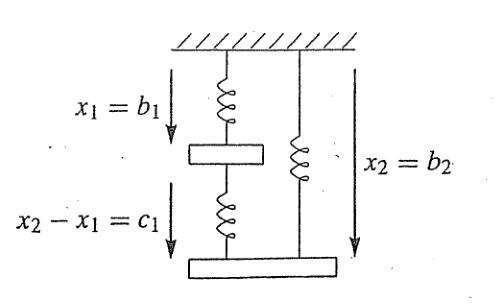
\includegraphics[width=0.7\linewidth]{TeX_files/Part02/chapter04/image/4-4}
		\caption{Figure 4.4 Mass-spring equivalent of the observation and state equations(4.32)}
	\end{figure}
	
	Kalman adds one spring at each prediction/correction.
	\begin{equation*}
	\hat{x}_{1|1}=b_1  \qquad  \hat{x}_{2|1}=b_1+c_1
	\end{equation*}
	\begin{equation*}
	\hat{x}_2=\hat{x}_{2|2}=\frac{1}{3}(b_1+2b_2+c_1)
	\end{equation*}
	
	Solution\; The (weighted) least squares principle for (4.30) still gives $\hat{x}_1$ and $\hat{x}_2$:
	\begin{equation}
	Minimize \quad
	E=\frac{1}{\sigma^2_1}(b_1-x_1)^2+\frac{1}{v^2_1}(c_1+x_1-x_2)^2+\frac{1}{\sigma^2_2}(b_2-x_2)^2
	\end{equation}
	The weighted normal equations $A^TCA=A^TCb$ will have $C^{-1}=diag(\sigma^2_1,v^2_1,\sigma^2_2)$. With $C=I,\sigma_1=\sigma_2=V_1=1$:
	\begin{equation}
	\begin{bmatrix}
	\hat{x}_1  \\ \hat{x}_2
	\end{bmatrix}
	 =
	\begin{bmatrix}
	b_1-c_1  \\  b_2+c_1
	\end{bmatrix}
	\end{equation}
	\begin{equation*}
	gives \quad
	\hat{x}_1=\frac{1}{3}(2b_1+b_2-c_1)
	\end{equation*}
	\begin{equation*}
	\quad
	\hat{x}_2=\frac{1}{3}(b_1+2b_2+c_1)
	\end{equation*}
	The latest estimate $\hat{x}_2$ gives a heavier weight $\frac{2}{3}$ to the latest measurement $b_2$.
	
	Now compute recursively. The key point is that $A^TCA$ is a tridiagonal matrix. (It
	will be block tridiagonal in Chapter 8 when the state x is a vector.) Measurement equations
	$A_ix_i=b_i$ are connected by state equations $x_{i+1}=F_ix_i+c_i$.	Forward elimination on
	the tridiagonal matrix $A^TCA$ is always a recursion for a multiplier and a pivot. Then
	back-substitution is a second recursion, backward in time.
	
	Key fact By itself, the forward recursion finds the best estimate of $\hat{x}_{i|i}$ based on measurements and state equations up to and including time t = i. Very often an estimate $\hat{x}_{n|n}$ of the final state is all we want. Then forget about back-substitution.
	
	The back-substitution step adjusts the earlier $\hat{x}_{i|i}$ to account for later measurements
	and state equations, after time i. Going back in this way is called “smoothing.” It produces
	the correct solutions $\hat{x}_{i|n}$ to the normal equations $A^TCA\hat{x}=A^TCb$.
	
	Even the forward recursion to find $\hat{x}_{i|i}$ is a two-step process. The previous
	$\hat{x}_{i-1|i-1}$ uses all information through time i - 1. The next state equation gives a prediction. Then the measurement $b_i$ adds a correction. Together Kalman's filter produces $\hat{x}_{i|i}$.
	\begin{equation*}
	Prediction \quad
	\hat{x}_{i|i-1}=F_{i-1}\hat{x}_{i-1|i-1}+c_i
	\end{equation*}
	\begin{equation*}
	Correction \quad
	\hat{x}_{i|i}=\hat{x}_{i|i-1}+K_i(b_i-A_i\hat{x}_{i|i-1})
	\end{equation*}
	That correction is written as an update using the gain matrix $K_i$. The new data are $c_i$ and $b_i$. We are solving the complete system Ax = b by least squares, adding in one equation at a
	time.
	
	As in recursive least squares, there is something more to compute — the confidence
	of our estimates $\hat{x}_{i|i}$. The covariance matrices $P_{i|i}=(A^TCA)^{-1}_i$
	are updated recursively too! Each Kalman filter step adds a (block) row to A and C, and a (block) column to $A^T$ and C. The prediction-correction steps compute $P_{i|i-1}$ and $P_{i|i}$, the variances of the errors in $\hat{x}_{i|i-1}$ amd $\hat{x}_{i|i}$.
	
	It is fair to say that the Kalman filter gets complicated, even if the plan is straightforward. All authors try to find a clear way to derive the matrix formulas for $\hat{x}_{i|i}$ and $P_{i|i}$. (There are multiple forms that give numerically different recursions.) Square-root filters using $LDL^T$ or QR were developed to reduce numerical instability when variances become very small or very large. Our exposition of the Kalman filter will come in Chapter 8.
	
	The essential point is that the covariance matrices $P_{i|i}$ have the same size as the
	states $x_i$. That size is independent of the number $m_i$ of measurements at step i. If we are
	updating the best fit by a straight line, our matrices remain 2 by 2.
	
	Example 4.7\; (Heart rates) Find P and $\hat{x}$ recursively, with C = I (unit variances):
	\begin{equation*}
	Start\, from\, x_1=b_1: \quad
	A_{1|1}=[1] \quad
	gives \quad
	P_{1|1}=(A^TA)^{-1}_{1|1}=[I]
	\end{equation*}
    \begin{equation*}
    Add\,x_2-x_1=c_1: \quad
    A_{2|1}=\begin{bmatrix} 1 & 0 \\ -1 & 1 \end{bmatrix}
    \quad and \quad
    (A^TA)^{-1}_{2|1}=\begin{bmatrix} 1 & 1 \\ 1 & 2 \end{bmatrix}
    \quad give \quad 
    P_{2|1}=2
    \end{equation*}
    \begin{equation*}
    include \,P_{2|1}=2: \quad
    A_{2|2}=\begin{bmatrix} -1 & 0 \\ -1 & 1 \\ 0 & 1 \end{bmatrix}
    \quad and \quad
    (A^TA)^{-1}_{2|2}=\frac{1}{3}\begin{bmatrix} 2 & 1 \\ 1 & 2 \end{bmatrix}
    \quad give \quad 
    P_{2|2}=\frac{2}{3}
    \end{equation*}	
	The first estimate is$\hat{x}_{1|1}=b_1$(not smoothed!). The next prediction is $\hat{x}_{2|1}=b_1+c_2$ using the state equation. The correction is $\frac{1}{3}(b_1+2b_2+c_1)$, , using the final $A_{2|2}$.
	
	Those variances $P_{2|1}=2$ and $P_{2|2}=\frac{2}{3}$ are the last entries in $(A^TA)^{-1}_{2|1}$ and $(A^TA)^{-1}_{2|2}$. Vectors $x_i$ lead to block pivots $P^{-1}$.
	Here 2 and $\frac{2}{3}$ are also seen as the sum of squares of	coefficients in $b_1+c_1$ and $\frac{1}{3}(b_1+2b_2+c_1)$.
	
	Back-substitution (smoothing) adjusts $\hat{x}_{1|1}=b_1$ to $\hat{x}_1=\frac{1}{3}(2b_1+b_2-c_1)$ as in (4.32).
	 
	
	
	
	
	
